\section{Introduction}\label{introduction}

\begin{frame}{Understanding and Describing Your Data}

We are going to take what we've learned from the previous two chapters
and use them together to have simple but powerful ways to understand
your data. This chapter will be broken down into:

\begin{enumerate}
\def\labelenumi{\arabic{enumi}.}
\tightlist
\item
  Descriptive Statistics
\item
  Visualizations
\end{enumerate}

The two go hand-in-hand in understanding what is happening in your data.

\end{frame}

\begin{frame}{Exploring Data}

We are often most interested in three things when exploring our data:

\begin{enumerate}
\def\labelenumi{\arabic{enumi}.}
\tightlist
\item
  \textbf{understanding distributions},
\item
  \textbf{understanding relationships}, and
\item
  \textbf{looking for outliers or errors}.
\end{enumerate}

\end{frame}

\section{Descriptive Statistics}\label{descriptive-statistics}

\begin{frame}[fragile]{Descriptive Statistics}

Several methods of discovering descriptives in a succinct way have been
developed for \texttt{R}.

\begin{itemize}
\tightlist
\item
  My favorite (full disclosure: it is one that I made so I may be
  biased) is the \texttt{table1} function in the \texttt{furniture}
  package.
\item
  It has been designed to be simple and complete.
\item
  It produces a well-formatted table that you can easily export and use
  as a table in a report or article.\footnote<.->{It is called
    ``table1'' because a nice descriptive table is often found in the
    first table of many academic papers.}
\end{itemize}

\end{frame}

\begin{frame}[fragile]{Table 1}

We'll first create a ficticious data set and we'll show the basic build
of \texttt{table1}.

\begin{Shaded}
\begin{Highlighting}[]
\KeywordTok{library}\NormalTok{(furniture)}
\NormalTok{df <-}\StringTok{ }\KeywordTok{data.frame}\NormalTok{(}\StringTok{"A"}\NormalTok{=}\KeywordTok{c}\NormalTok{(}\DecValTok{1}\NormalTok{,}\DecValTok{2}\NormalTok{,}\DecValTok{1}\NormalTok{,}\DecValTok{4}\NormalTok{,}\DecValTok{3}\NormalTok{,}\OtherTok{NA}\NormalTok{),}
                 \StringTok{"B"}\NormalTok{=}\KeywordTok{c}\NormalTok{(}\FloatTok{1.4}\NormalTok{,}\FloatTok{2.1}\NormalTok{,}\FloatTok{4.6}\NormalTok{,}\FloatTok{2.0}\NormalTok{,}\OtherTok{NA}\NormalTok{,}\FloatTok{3.4}\NormalTok{),}
                 \StringTok{"C"}\NormalTok{=}\KeywordTok{c}\NormalTok{(}\DecValTok{0}\NormalTok{,}\DecValTok{0}\NormalTok{,}\DecValTok{1}\NormalTok{,}\DecValTok{1}\NormalTok{,}\DecValTok{1}\NormalTok{,}\DecValTok{1}\NormalTok{),}
                 \StringTok{"D"}\NormalTok{=}\KeywordTok{rnorm}\NormalTok{(}\DecValTok{6}\NormalTok{))}
\end{Highlighting}
\end{Shaded}

\end{frame}

\begin{frame}[fragile]{Table 1}

This can quickly give you means and standard deviations (or counts and
percentages for categorical variables).

``A'' and ``C'' are supposed to be factors in this fake data set.

\begin{Shaded}
\begin{Highlighting}[]
\NormalTok{df}\OperatorTok{$}\NormalTok{A <-}\StringTok{ }\KeywordTok{factor}\NormalTok{(df}\OperatorTok{$}\NormalTok{A, }\DataTypeTok{labels=}\KeywordTok{c}\NormalTok{(}\StringTok{"cat1"}\NormalTok{, }\StringTok{"cat2"}\NormalTok{, }\StringTok{"cat3"}\NormalTok{, }\StringTok{"cat4"}\NormalTok{))}
\NormalTok{df}\OperatorTok{$}\NormalTok{C <-}\StringTok{ }\KeywordTok{factor}\NormalTok{(df}\OperatorTok{$}\NormalTok{C, }\DataTypeTok{labels=}\KeywordTok{c}\NormalTok{(}\StringTok{"male"}\NormalTok{, }\StringTok{"female"}\NormalTok{))}
\end{Highlighting}
\end{Shaded}

\end{frame}

\begin{frame}[fragile]{Table 1}

Then we can use \texttt{table1()}.

\begin{Shaded}
\begin{Highlighting}[]
\KeywordTok{table1}\NormalTok{(df, A, B, C, D)}
\end{Highlighting}
\end{Shaded}

\begin{verbatim}

|==============================|
              Mean/Count (SD/%)
 Observations 6                
 A                             
    cat1      2 (40%)          
    cat2      1 (20%)          
    cat3      1 (20%)          
    cat4      1 (20%)          
 B                             
              2.7 (1.3)        
 C                             
    male      2 (33.3%)        
    female    4 (66.7%)        
 D                             
              -0.2 (0.5)       
|==============================|
\end{verbatim}

\end{frame}

\begin{frame}[fragile]{Table 1}

So now we see the counts and percentages for the factor variables. But
now we can take a step further and look for relationships. The code
below shows the means/standard devaitions or counts/percentages by a
grouping variable--in this case, \texttt{C}.

\begin{Shaded}
\begin{Highlighting}[]
\KeywordTok{table1}\NormalTok{(df, A, B, D,}
       \DataTypeTok{splitby =} \OperatorTok{~}\NormalTok{C)}
\end{Highlighting}
\end{Shaded}

\begin{verbatim}

|=================================|
                  C 
              male      female    
 Observations 2         4         
 A                                
    cat1      1 (50%)   1 (33.3%) 
    cat2      1 (50%)   0 (0%)    
    cat3      0 (0%)    1 (33.3%) 
    cat4      0 (0%)    1 (33.3%) 
 B                                
              1.8 (0.5) 3.3 (1.3) 
 D                                
              0.1 (0.8) -0.3 (0.3)
|=================================|
\end{verbatim}

\end{frame}

\begin{frame}[fragile]{Table 1}

We can also test for differences by group as well (although this is not
particularly good with a sample size of 5). It produces a warning since
the \(\chi^2\) approximation is not accurate with cells this small.

\begin{Shaded}
\begin{Highlighting}[]
\KeywordTok{table1}\NormalTok{(df, A, B, D,}
       \DataTypeTok{splitby =} \OperatorTok{~}\NormalTok{C,}
       \DataTypeTok{test=}\OtherTok{TRUE}\NormalTok{)}
\end{Highlighting}
\end{Shaded}

\begin{verbatim}

|=========================================|
                      C 
              male      female     P-Value
 Observations 2         4                 
 A                                 0.405  
    cat1      1 (50%)   1 (33.3%)         
    cat2      1 (50%)   0 (0%)            
    cat3      0 (0%)    1 (33.3%)         
    cat4      0 (0%)    1 (33.3%)         
 B                                 0.162  
              1.8 (0.5) 3.3 (1.3)         
 D                                 0.605  
              0.1 (0.8) -0.3 (0.3)        
|=========================================|
\end{verbatim}

\end{frame}

\begin{frame}[fragile]{Table 1}

Finally, we can play around with the formatting a bit to match what we
need:

\begin{Shaded}
\begin{Highlighting}[]
\KeywordTok{table1}\NormalTok{(df, A, B, D,}
       \DataTypeTok{splitby =} \OperatorTok{~}\NormalTok{C,}
       \DataTypeTok{test=}\OtherTok{TRUE}\NormalTok{,}
       \DataTypeTok{type =} \KeywordTok{c}\NormalTok{(}\StringTok{"simple"}\NormalTok{, }\StringTok{"condense"}\NormalTok{))}
\end{Highlighting}
\end{Shaded}

\begin{verbatim}

|=========================================|
                      C 
              male      female     P-Value
 Observations 2         4                 
 A                                 0.405  
    cat1      50%       33.3%             
    cat2      50%       0%                
    cat3      0%        33.3%             
    cat4      0%        33.3%             
 B            1.8 (0.5) 3.3 (1.3)  0.162  
 D            0.1 (0.8) -0.3 (0.3) 0.605  
|=========================================|
\end{verbatim}

\end{frame}

\begin{frame}[fragile]{Table 1}

So with three or four short lines of code we can get a good idea about
variables that may be related to the grouping variable and any
missingness in the factor variables. There's much more you can do with
\texttt{table1} and there are vignettes and tutorials available to learn
more.\footnote<.->{\url{tysonstanley.github.io}}

\end{frame}

\begin{frame}[fragile]{Other Descriptive Functions}

Other quick descriptive functions exist; here are a few of them.

\begin{Shaded}
\begin{Highlighting}[]
\KeywordTok{summary}\NormalTok{(df)          ## descriptives for each variable in the data}

\KeywordTok{library}\NormalTok{(psych)       ## install first}
\KeywordTok{describe}\NormalTok{(df)         ## produces summary statistics for continuous variables}

\KeywordTok{library}\NormalTok{(Hmisc)       ## install first}
\NormalTok{Hmisc}\OperatorTok{::}\KeywordTok{describe}\NormalTok{(df)  ## gives summary for each variable separately}
\end{Highlighting}
\end{Shaded}

\end{frame}

\section{Visualizations}\label{visualizations}

\begin{frame}{Visualizations}

Understanding your data, in my experience, generally requires
visualizations.

Can help us:

\begin{itemize}
\tightlist
\item
  understand the distributions and relationships
\item
  catch errors in the data
\item
  find any outliers that could be highly influencing any models
\end{itemize}

\end{frame}

\begin{frame}[fragile]{\texttt{ggplot2}}

For simple but appealing visualizations we are going to be using
\texttt{ggplot2}.

\begin{quote}
This package is used to produce professional level plots for many
journalism organizations (e.g.~five-thrity-eight). These plots are
quickly presentation quality and can be used to impress your boss, your
advisor, or your friends.
\end{quote}

\end{frame}

\begin{frame}[fragile]{\texttt{ggplot2}}

This package has a straight-forward syntax. It is built by adding layers
to the plot.

\begin{Shaded}
\begin{Highlighting}[]
\KeywordTok{library}\NormalTok{(ggplot2)   ## first install using install.packages("ggplot2")}
\end{Highlighting}
\end{Shaded}

\end{frame}

\begin{frame}[fragile]{\texttt{ggplot2}}

First, we have a nice \texttt{qplot} function that provides us a ``quick
plot.'' It quickly decides what kind of plot is useful given the data
and variables you provide.

\begin{Shaded}
\begin{Highlighting}[]
\KeywordTok{qplot}\NormalTok{(df}\OperatorTok{$}\NormalTok{A)  ## Makes a simple histogram}
\end{Highlighting}
\end{Shaded}

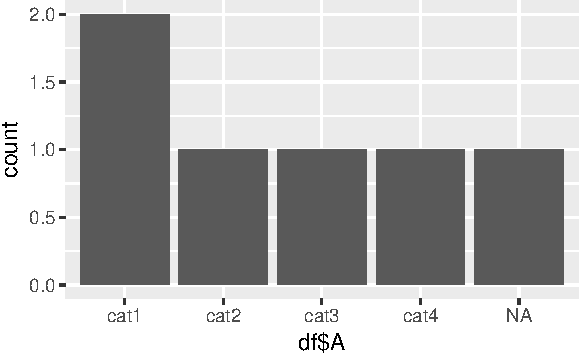
\includegraphics{03_UnderstandData_files/figure-beamer/unnamed-chunk-9-1.pdf}

\end{frame}

\begin{frame}[fragile]{\texttt{ggplot2}}

\begin{Shaded}
\begin{Highlighting}[]
\KeywordTok{qplot}\NormalTok{(df}\OperatorTok{$}\NormalTok{D, df}\OperatorTok{$}\NormalTok{B)  ## Makes a scatterplot}
\end{Highlighting}
\end{Shaded}

\begin{verbatim}
Warning: Removed 1 rows containing missing values (geom_point).
\end{verbatim}

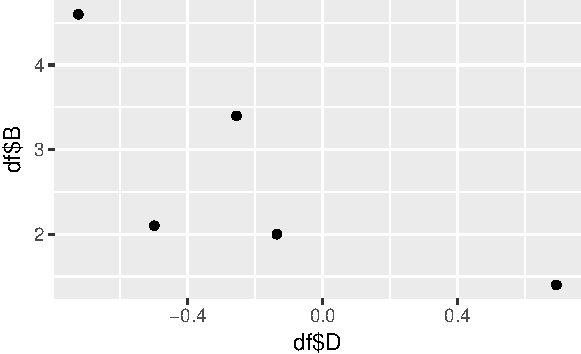
\includegraphics{03_UnderstandData_files/figure-beamer/unnamed-chunk-10-1.pdf}

\end{frame}

\begin{frame}[fragile]{\texttt{ggplot2}}

For a bit more control over the plot, you can use the \texttt{ggplot}
function. The first piece is the \texttt{ggplot} piece. From there, we
add layers. These layers generally start with \texttt{geom\_} then have
the type of plot.

\end{frame}

\begin{frame}[fragile]{\texttt{ggplot2}}

Below, we start with telling \texttt{ggplot} the basics of the plot and
then build a boxplot. The x-axis is the variable ``C'' and the y-axis is
the variable ``D'' and then we color it by variable ``C'' as well.

\begin{Shaded}
\begin{Highlighting}[]
\KeywordTok{ggplot}\NormalTok{(df, }\KeywordTok{aes}\NormalTok{(}\DataTypeTok{x=}\NormalTok{C, }\DataTypeTok{y=}\NormalTok{D)) }\OperatorTok{+}
\StringTok{  }\KeywordTok{geom_boxplot}\NormalTok{(}\KeywordTok{aes}\NormalTok{(}\DataTypeTok{color =}\NormalTok{ C))}
\end{Highlighting}
\end{Shaded}

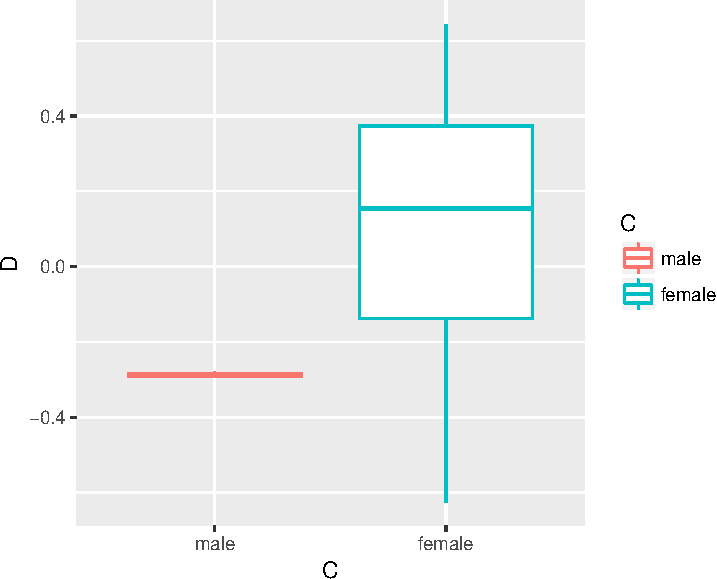
\includegraphics{03_UnderstandData_files/figure-beamer/unnamed-chunk-11-1.pdf}

\end{frame}

\begin{frame}[fragile]{\texttt{ggplot2}}

Here are a few more examples:

\begin{Shaded}
\begin{Highlighting}[]
\KeywordTok{ggplot}\NormalTok{(df, }\KeywordTok{aes}\NormalTok{(}\DataTypeTok{x=}\NormalTok{C)) }\OperatorTok{+}
\StringTok{  }\KeywordTok{geom_bar}\NormalTok{(}\DataTypeTok{stat=}\StringTok{"count"}\NormalTok{, }\KeywordTok{aes}\NormalTok{(}\DataTypeTok{fill =}\NormalTok{ C))}
\end{Highlighting}
\end{Shaded}

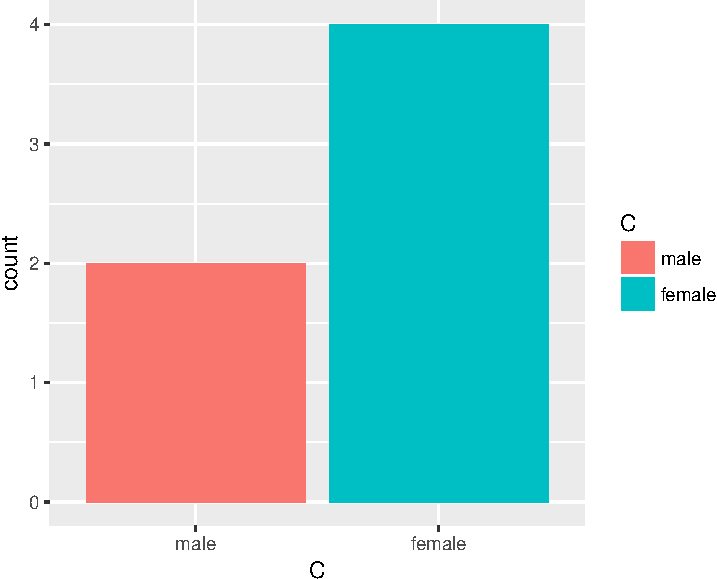
\includegraphics{03_UnderstandData_files/figure-beamer/unnamed-chunk-12-1.pdf}

\end{frame}

\begin{frame}[fragile]{\texttt{ggplot2}}

\begin{Shaded}
\begin{Highlighting}[]
\KeywordTok{ggplot}\NormalTok{(df, }\KeywordTok{aes}\NormalTok{(}\DataTypeTok{x=}\NormalTok{B, }\DataTypeTok{y=}\NormalTok{D)) }\OperatorTok{+}
\StringTok{  }\KeywordTok{geom_point}\NormalTok{(}\KeywordTok{aes}\NormalTok{(}\DataTypeTok{color =}\NormalTok{ C))}
\end{Highlighting}
\end{Shaded}

\begin{verbatim}
Warning: Removed 1 rows containing missing values (geom_point).
\end{verbatim}

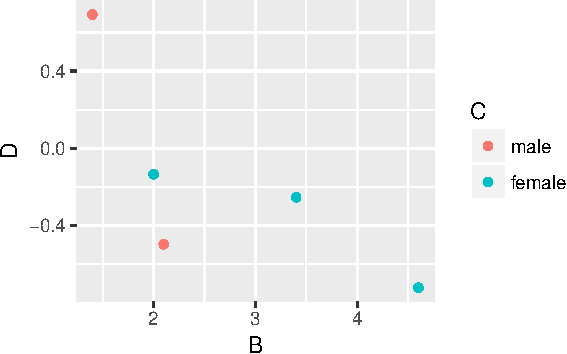
\includegraphics{03_UnderstandData_files/figure-beamer/unnamed-chunk-13-1.pdf}
\emph{Note that the warning that says it removed a row is because we had
a missing value in ``C''.}

\end{frame}

\begin{frame}[fragile]{\texttt{ggplot2}}

We are going to make the first one again but with some aesthetic
adjustments. Notice that we just added two extra lines telling
\texttt{ggplot2} how we want some things to look.\footnote<.->{This is
  just scratching the surface of what we can change in the plots.}

\end{frame}

\begin{frame}[fragile]{A final example}

\begin{Shaded}
\begin{Highlighting}[]
\KeywordTok{ggplot}\NormalTok{(df, }\KeywordTok{aes}\NormalTok{(}\DataTypeTok{x=}\NormalTok{C, }\DataTypeTok{y=}\NormalTok{D)) }\OperatorTok{+}
\StringTok{  }\KeywordTok{geom_boxplot}\NormalTok{(}\KeywordTok{aes}\NormalTok{(}\DataTypeTok{color =}\NormalTok{ C)) }\OperatorTok{+}
\StringTok{  }\KeywordTok{theme_bw}\NormalTok{() }\OperatorTok{+}
\StringTok{  }\KeywordTok{scale_color_manual}\NormalTok{(}\DataTypeTok{values =} \KeywordTok{c}\NormalTok{(}\StringTok{"dodgerblue4"}\NormalTok{, }\StringTok{"coral2"}\NormalTok{))}
\end{Highlighting}
\end{Shaded}

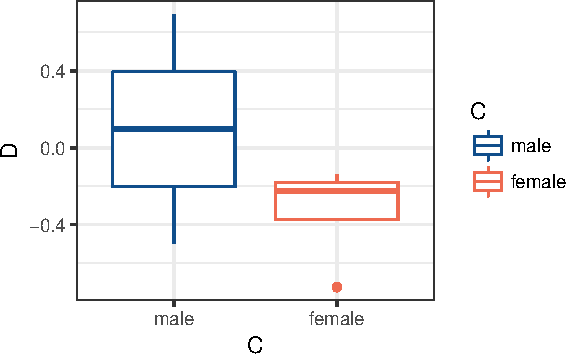
\includegraphics{03_UnderstandData_files/figure-beamer/unnamed-chunk-14-1.pdf}

\end{frame}

\begin{frame}[fragile]{A final example}

\begin{itemize}
\tightlist
\item
  \texttt{theme\_bw()} makes the background white,
\item
  the \texttt{scale\_color\_manual()} allows us to change the colors in
  the plot.
\end{itemize}

You can get a good idea of how many types of plots you can do by going
to
\href{http://docs.ggplot2.org/current/}{http://docs.ggplot2.org/current}.

Almost any informative plot that you need to do as a researcher is
possible with \texttt{ggplot2}.

We will be using \texttt{ggplot2} extensively in the class to help
understand our data and our models as well as communicate our results.

\end{frame}

\begin{frame}

\centerline{
\includegraphics[height=7in]{Figures/grass_landscape_arch.jpg}}

\end{frame}
